\documentclass{sigchi}

% Use this command to override the default ACM copyright statement
% (e.g. for preprints).  Consult the conference website for the
% camera-ready copyright statement.

%% EXAMPLE BEGIN -- HOW TO OVERRIDE THE DEFAULT COPYRIGHT STRIP -- (July 22, 2013 - Paul Baumann)
% \toappear{Permission to make digital or hard copies of all or part of this work for personal or classroom use is      granted without fee provided that copies are not made or distributed for profit or commercial advantage and that copies bear this notice and the full citation on the first page. Copyrights for components of this work owned by others than ACM must be honored. Abstracting with credit is permitted. To copy otherwise, or republish, to post on servers or to redistribute to lists, requires prior specific permission and/or a fee. Request permissions from permissions@acm.org. \\
% {\emph{CHI'14}}, April 26--May 1, 2014, Toronto, Canada. \\
% Copyright \copyright~2014 ACM ISBN/14/04...\$15.00. \\
% DOI string from ACM form confirmation}
%% EXAMPLE END -- HOW TO OVERRIDE THE DEFAULT COPYRIGHT STRIP -- (July 22, 2013 - Paul Baumann)

% Arabic page numbers for submission.  Remove this line to eliminate
% page numbers for the camera ready copy
% \pagenumbering{arabic}

% Load basic packages
\usepackage{balance}  % to better equalize the last page
\usepackage{graphics} % for EPS, load graphicx instead 
\usepackage[T1]{fontenc}
\usepackage{txfonts}
\usepackage{mathptmx}
\usepackage[pdftex]{hyperref}
\usepackage{color}
\usepackage{booktabs}
\usepackage{textcomp}
% Some optional stuff you might like/need.
\usepackage{microtype} % Improved Tracking and Kerning
% \usepackage[all]{hypcap}  % Fixes bug in hyperref caption linking
\usepackage{ccicons}  % Cite your images correctly!
% \usepackage[utf8]{inputenc} % for a UTF8 editor only

% If you want to use todo notes, marginpars etc. during creation of your draft document, you
% have to enable the "chi_draft" option for the document class. To do this, change the very first
% line to: "\documentclass[chi_draft]{sigchi}". You can then place todo notes by using the "\todo{...}"
% command. Make sure to disable the draft option again before submitting your final document.
\usepackage{todonotes}

% Paper metadata (use plain text, for PDF inclusion and later
% re-using, if desired).  Use \emtpyauthor when submitting for review
% so you remain anonymous.
\def\plaintitle{Synthetic Interviewing with Semantic Search}
\def\plainauthor{First Author, Second Author, Third Author,
  Fourth Author, Fifth Author, Sixth Author}
\def\emptyauthor{}
\def\plainkeywords{Authors' choice; of terms; separated; by
  semicolons; include commas, within terms only; required.}
\def\plaingeneralterms{Documentation, Standardization}

% llt: Define a global style for URLs, rather that the default one
\makeatletter
\def\url@leostyle{%
  \@ifundefined{selectfont}{
    \def\UrlFont{\sf}
  }{
    \def\UrlFont{\small\bf\ttfamily}
  }}
\makeatother
\urlstyle{leo}

% To make various LaTeX processors do the right thing with page size.
\def\pprw{8.5in}
\def\pprh{11in}
\special{papersize=\pprw,\pprh}
\setlength{\paperwidth}{\pprw}
\setlength{\paperheight}{\pprh}
\setlength{\pdfpagewidth}{\pprw}
\setlength{\pdfpageheight}{\pprh}

% Make sure hyperref comes last of your loaded packages, to give it a
% fighting chance of not being over-written, since its job is to
% redefine many LaTeX commands.
\definecolor{linkColor}{RGB}{6,125,233}
\hypersetup{%
  pdftitle={\plaintitle},
% Use \plainauthor for final version.
%  pdfauthor={\plainauthor},
  pdfauthor={\emptyauthor},
  pdfkeywords={\plainkeywords},
  bookmarksnumbered,
  pdfstartview={FitH},
  colorlinks,
  citecolor=black,
  filecolor=black,
  linkcolor=black,
  urlcolor=linkColor,
  breaklinks=true,
}

% create a shortcut to typeset table headings
% \newcommand\tabhead[1]{\small\textbf{#1}}

% End of preamble. Here it comes the document.
\begin{document}

\title{\plaintitle}

\numberofauthors{3}
\author{%
  \alignauthor{Leave Authors Anonymous\\
    \affaddr{for Submission}\\
    \affaddr{City, Country}\\
    \email{e-mail address}}\\
  \alignauthor{Leave Authors Anonymous\\
    \affaddr{for Submission}\\
    \affaddr{City, Country}\\
    \email{e-mail address}}\\
  \alignauthor{Leave Authors Anonymous\\
    \affaddr{for Submission}\\
    \affaddr{City, Country}\\
    \email{e-mail address}}\\
}

\maketitle

\begin{abstract}
  In this paper we describe a novel tool to open up new windows of exploration for qualitative researchers. Through the use of semantic search algorithms applied to a large corpus of data, obtained from LiveJournal.com, we are able to extract valuable information that qualitative researchers can use in their methodology. We describe the design processes that lead us to the development of this tool. We analyze the results of an open user study with qualitative researchers, which helped us confirm the value of the tool and lead to the development of additional features. Finally we present comparisons between results obtained by modifying certain input parameters such as: percentage of data used, number of results returned, filtering, and word weighting.
\end{abstract}

\category{H.5.m.}{Information Interfaces and Presentation
  (e.g. HCI)}{Miscellaneous} \category{See
  \url{http://acm.org/about/class/1998/} for the full list of ACM
  classifiers. This section is required.}{}{}

\keywords{semantic search; big data; qualitative; ethnography; synthetic; methods}

\section{Introduction}

Imagine a huge library filled with millions of personal diaries. 

The use of big data in the qualitative research community has increased quite a bit in recent years. From Twitter sentiment inference [AA] to semantic research corpus data search tools [BB] there are more and more efforts being made to extract meaning from large corpus of text data. Our approach is to take advantage of modern algorithms such as word2vec, which transform words into high dimensional vectors (typically 300) and perform arithmetic operations in this basis coordinates. For example, (the vector for the word) ?king? minus the word ?man? plus the word ?woman? equals to ?queen?.

\section{Methodology}

\subsection{LiveJournal Corpus}
For this study we were able to obtain a data set consisting of all LiveJournal posts as of November 2012 in raw XML format. LiveJournal is a social networking service where users can keep a blog, journal, or diary. Users have their own journal pages, which show all of their most recent journal entries. Each journal entry can also be viewed on its own web page which includes comments left by other users. 

LiveJournal in the United States currently receives about 170 million page views each month from 10 million unique visitors. Our data contains about one million users with a total of 64,326,865 text posts. Of the users that provided their date of birth, the majority were in the 17-25 age group. Users were able to indicate their binary gender; of those who did so 45\% identified as male and 55\% as female. 

\subsection{Data preprocessing}

We started with a raw XML dataset which consists of more than nine billion words in over 500 million sentences. In order to extract semantic meaning and run synthetic interviews through the use of natural language processing (NLP) algorithms, we implemented a data pipeline that allows us to extract and clean the post text in a computationally efficient form. 

The first step is to tokenize the corpus using FLEX (Fast Lexical Analyzer), a scanner which maps each word in the corpus to a unique number and saves the mapping in a dictionary. For efficiency, we keep only the 994,949 most common words and discard the rest (all of which occur fewer than 41 times in the entire dataset). Care is taken to properly tokenize numbers and emoticons such as ``:-)'', ``=<'' or ``>:P''.

After removing non-textual content such as images, hyperlinks, and XML formatting data, a bag of words representation is saved for each sentence from the posts as a column in a sparse feature matrix. The rows correspond to the entries in the dictionary above, and the values in the matrix are the counts of each entry for each sentence. For each sentence, we also store the id of the post it belongs to and the user who wrote it so that the original post can be found online. Finally, we need the sentence itself so that we can show it in the results when performing the query.

%The first thing we implemented was Lucene search into our dataset. This allowed us to first actually see what users were writing and with what moods. UCSF School of Nursing has a life events questionnaire detailing < http://nursing.ucsf.edu/sites/nursing.ucsf.edu/files/LifeEventsQues.pdf> ten categories of life events that may bring about changes in the lives of those who experience them. Some major categories are health, work, love and marriage, family and close friends, personal and social. We wanted to search through the data and see the posts relating to major life events such as disease, cancer, and others. 

\subsection{word2vec}

We will begin our exploration towards synthetic interviewing by employing a popular word embedding model called word2vec \cite{Mikolov2013,MikolovSCCD13} which has been successful in a variety of NLP applications including analogy tasks, sentence completion, machine translation \cite{W15-4908}, and topic modelling \cite{djuric2015hierarchical}. Word embedding models map each word of a dictionary to a lower dimensional continuous vector representation. With word2vec, this embedding is learned automatically from a sample corpus using a recurrent neural network. 

The true power of the technique is that the resulting feature space demonstrates semantic structure, i.e. it has been shown that vec(``king'') - vec(``man'') + vec(``woman'') has a greater cosine similarity to vec(``queen'') than to the vector of any other word in the dictionary. We can also generalize this comparison technique beyond the scope of single-words. By performing vector addition on the word vector embeddings of corresponding words and normalizing the resulting sum, we can compare the semantic proximity of complete sentences. This procedure is described in detail below.

We use two embedding models. First, we train our own embedding model on the corpus of LiveJournal posts using the Skip-gram with negative sampling (SGNS) implementation of word2vec as recommended in \cite{MikolovSCCD13}. This model gives 300-dimensional embeddings for the 994,949 words in our dictionary. Conveniently, Mikolov et al published a pre-trained SGNS word2vec model for open source access \cite{word2vecWEB}. This model was trained on an approximately 100 billion-word Google News corpus, and gives 300-dimensional embeddings for 3 million unique words. All of the words from our LiveJournal dictionary that are not included in this model can be assumed to map to zero vectors. Common stop words (i.e. ``the", ``an", ``who'') are also mapped to zero vectors, as they provide little semantic information.  

\begin{figure}[tb]
\centering 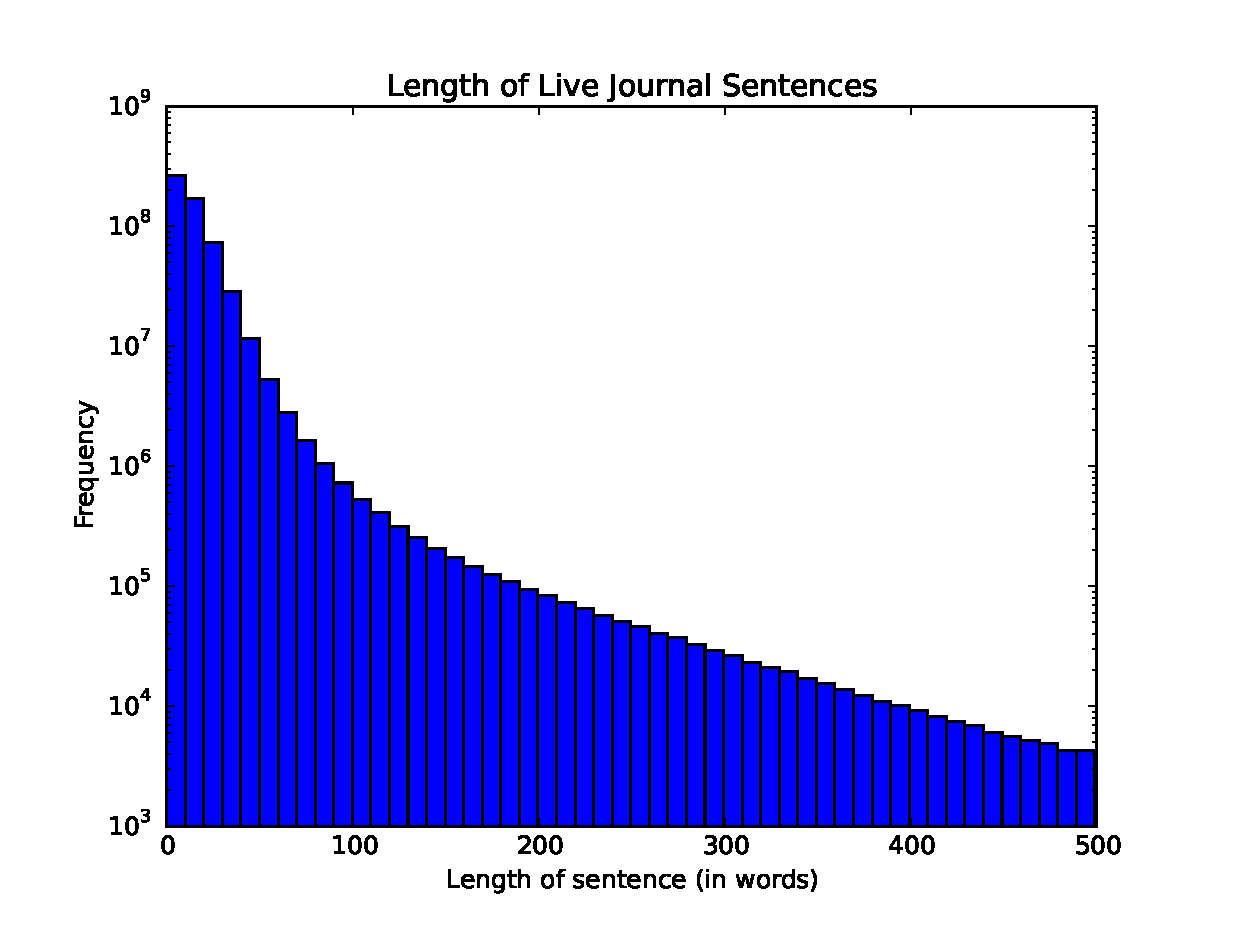
\includegraphics[width=0.5\textwidth]{figures/LJCounts} 
\caption{Histogram of the distribution of sentence lengths in the LiveJournal dataset. \label{fig:wordCounts}}
\end{figure}

\begin{figure}[tb]
\centering 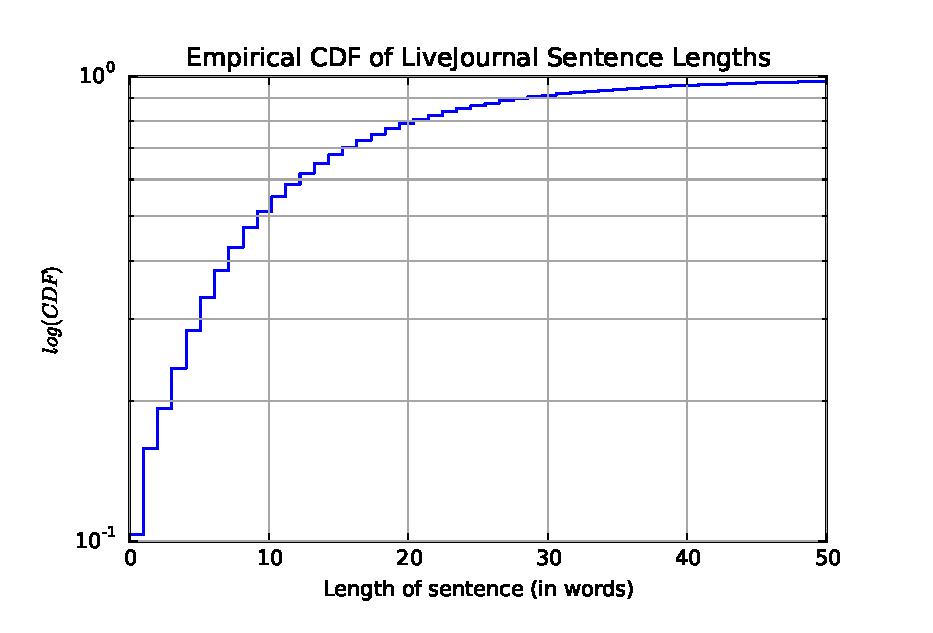
\includegraphics[width=0.5\textwidth]{figures/wordCDF} 
\caption{Cumulative distribution function for the distribution of sentence lengths in the LiveJournal dataset which represents the percentage of sentences containing less than a given number of words. Note that the $y$-axis is logarithmic. \label{fig:wordCDF}}
\end{figure}

\subsection{Querying}

Our goal is to perform semantic searches on the dataset from queries which can be phrased naturally as a sentence. To do this, we require a procedure for mapping sentences to the word vector space so that the cosine similarity still makes sense. We do this by first normalizing the rows of the embedding matrix, so that each word in the dictionary has the same norm. A sentence is then embedded by summing the projections of each constituent word. 

In order to query the data, we multiply the word2vec embedding matrix and the sparse bag of words matrix described above to get a semantic matrix. Each column of this matrix is the word2vec semantic encoding of a sentence in our data set. We divide each column by its norm, so that the magnitude of each column is 1 regardless of the number of words in the sentence. This allows us to perform queries simply by performing the dot product of each column with the query vector. The sentences with the largest inner product scores have the strongest semantic match to the query. We display a certain number of these sentences, which we call the responses to the query, for the user.

Although the system above gives us valuable information, we will see in the following section that some additional features are helpful to tune the responses and obtain more qualitatively interesting responses. First, we use a minimum {\em threshold} on the number of words in the response. No response is allowed which contains fewer words than the threshold. All words, including stop words and out-of-dictionary words, are included in this total. Figure~\ref{fig:wordCounts} shows the distribution of sentence lengths, thereby informing how such a cut will reduce the number of sentences available to query. 

Second, the user is given the power to {\em filter} responses which contain a specific word (or a word from a specific set). No sentence  containing one or more words from the set of filter words is returned in this case. One simple case in which this is helpful is to suppress responses with exact matches to words from the query.

We also give the user the ability to add {\em importance weighting} to words in the search query. In this case, when finding the embedding of the query sentence we multiply the contribution of the individual words by their importance weights before summing and normalizing. Note that these weights can be positive or negative. In the latter case responses with semantic relation to the negatively weighted word are suppressed.

\section{Results}

\subsection{Bridging Formal with Informal Language}
By applying the discussed SGNS Google News-trained word2vec model, on our LiveJournal sparse matrix, we simulate a bridge between formal semantics and vast compilation of informal anecdotes. To explore the potential advantage of such combination, we extended this tool to several academic researchers. As stated by an academic (insert\_name\_1), he/she states that ?the tool allows researchers to rapidly analyze an informal corpus ? one that has been previously hard to search?. (I am hoping we have transcripts that echo something along these lines). In such instances, we began validating the usability of synthetic interviewing for academic research. To demonstrate examples, we can observe (insert\_name\_1?s) 
results when querying topics relating to atkins diet.  (insert\_diagram\_of\_results\_of\_diet\_query\_here) In another instance, (insert\_name\_2) of (some\_other\_field), ran queries and yielded similar results. (insert\_diagram\_of\_results\_of\_family\_query\_here). 

The obtained results demonstrate one of many applications of generating synthetic interviews. This inspires curiosity of finding ways to expand its relevance beyond an academic setting. 

\subsection{Model versus Corpus}
While a majority of our trials yielded positive results, we cannot ignore the remaining minority that did not echo similar success. [insert\_example\_of\_unsucessful\_results\_here]

Such subpar retrievals bring attention to the parameters that may impact the quality of our queries. There are two major variables we chose in our implementation: the text corpus for training (Google News) and the actual corpus of text we are querying on (LiveJournal). In many cases, we found our choices to be sufficient; in an academic context, we can imagine researchers to seek answers to formal questions, in order to trigger responses that may be colloquial anecdotes. However, as demonstrated by the [failed\_attempt], an appropriate training-query corpus pair for one category may not necessarily be optimal for another category.

To find such pair that is appropriate for a desired topic, we recognize that there are distinct trends and biases from corpus to corpus. In our case, we observed that a dominating majority of the posts were in the form of journal entries, as LiveJournal was designed for that purpose. And most authors were within the 17-25 age group. Furthermore, we noticed from our bag-of-words model that topics frequently discussed included [list of frequent topics]. 

By understanding these properties, we can???. [to be continued] 


\subsection{EVALUATION}
We interviewed 5 researchers who worked on the tool generating queries. Initially

\section{Conclusions}


\section{Acknowledgments}

Sample text: We thank all the volunteers, and all publications support
and staff, who wrote and provided helpful comments on previous
versions of this document. Authors 1, 2, and 3 gratefully acknowledge
the grant from NSF (\#1234--2012--ABC). \textit{This whole paragraph is
  just an example.}


\bibliographystyle{SIGCHI-Reference-Format}
\bibliography{destressCHI}

\end{document}
